%!TEX root = ../ausarbeitung.tex
\newpage
\section{Klassifizierung mit Histograms of Gradients und Support Vector Machines}

\subsection{Kurzeinführung zu Histograms of Oriented Gradients}

Die Bezeichnung \textit{Histograms of Oriented Gradients} (HOG) bezeichnet einen \textit{Feature Descriptor} und wurde bekannt durch die Arbeit von Navneet Dalal and Bill Triggs \cite{dalal05}. Initial wurde der Deskriptor verwendet um Fußgänger zu detektieren. Später wurde er auch für andere Objekte wie Autos, Busse und Tiere eingesetzt. Wie der Name bereits andeutet handelt es sich bei HOG um ein Histogramm basierten \textit{Feature Descriptor}. Die Berechnung des HOG-Descriptors lässt sich in drei Schritte unterteilen: Gradientenberechnung, Gruppierung der Orientierungen und Histogrammerzeugung. Häufig werden  auch Vorverarbeitungsschritte, wie zum Beispiel ein Histogrammausgleich durchgeführt.

Zur Gradientenberechnung wird der Sobel-Operator verwendet. Eine visuelle Darstellung des Ergebnisses ist in Abbildung~\ref{fig:sobel} gezeigt. Zu sehen ist die Magnitude der Ableitung über die vertikale (links) und horizontale (rechts) Bildachse. Dabei entspricht in dieser Darstellung der Grauwert der positiv definierten Magnitude des Gradienten. Mit den folgenden Formeln lassen sich aus den Beiden Gradienten die positiv definierte gesamt Magnitude $|G|$ und die Orientierung $\Theta$ berechnen:  

\begin{equation}
|G| = \sqrt{G_x^2 + G_y^2}
\end{equation}
\begin{equation}
\Theta = \arctan({G_x, G_y})
\end{equation}

\begin{center}
\begin{tabular}{c}
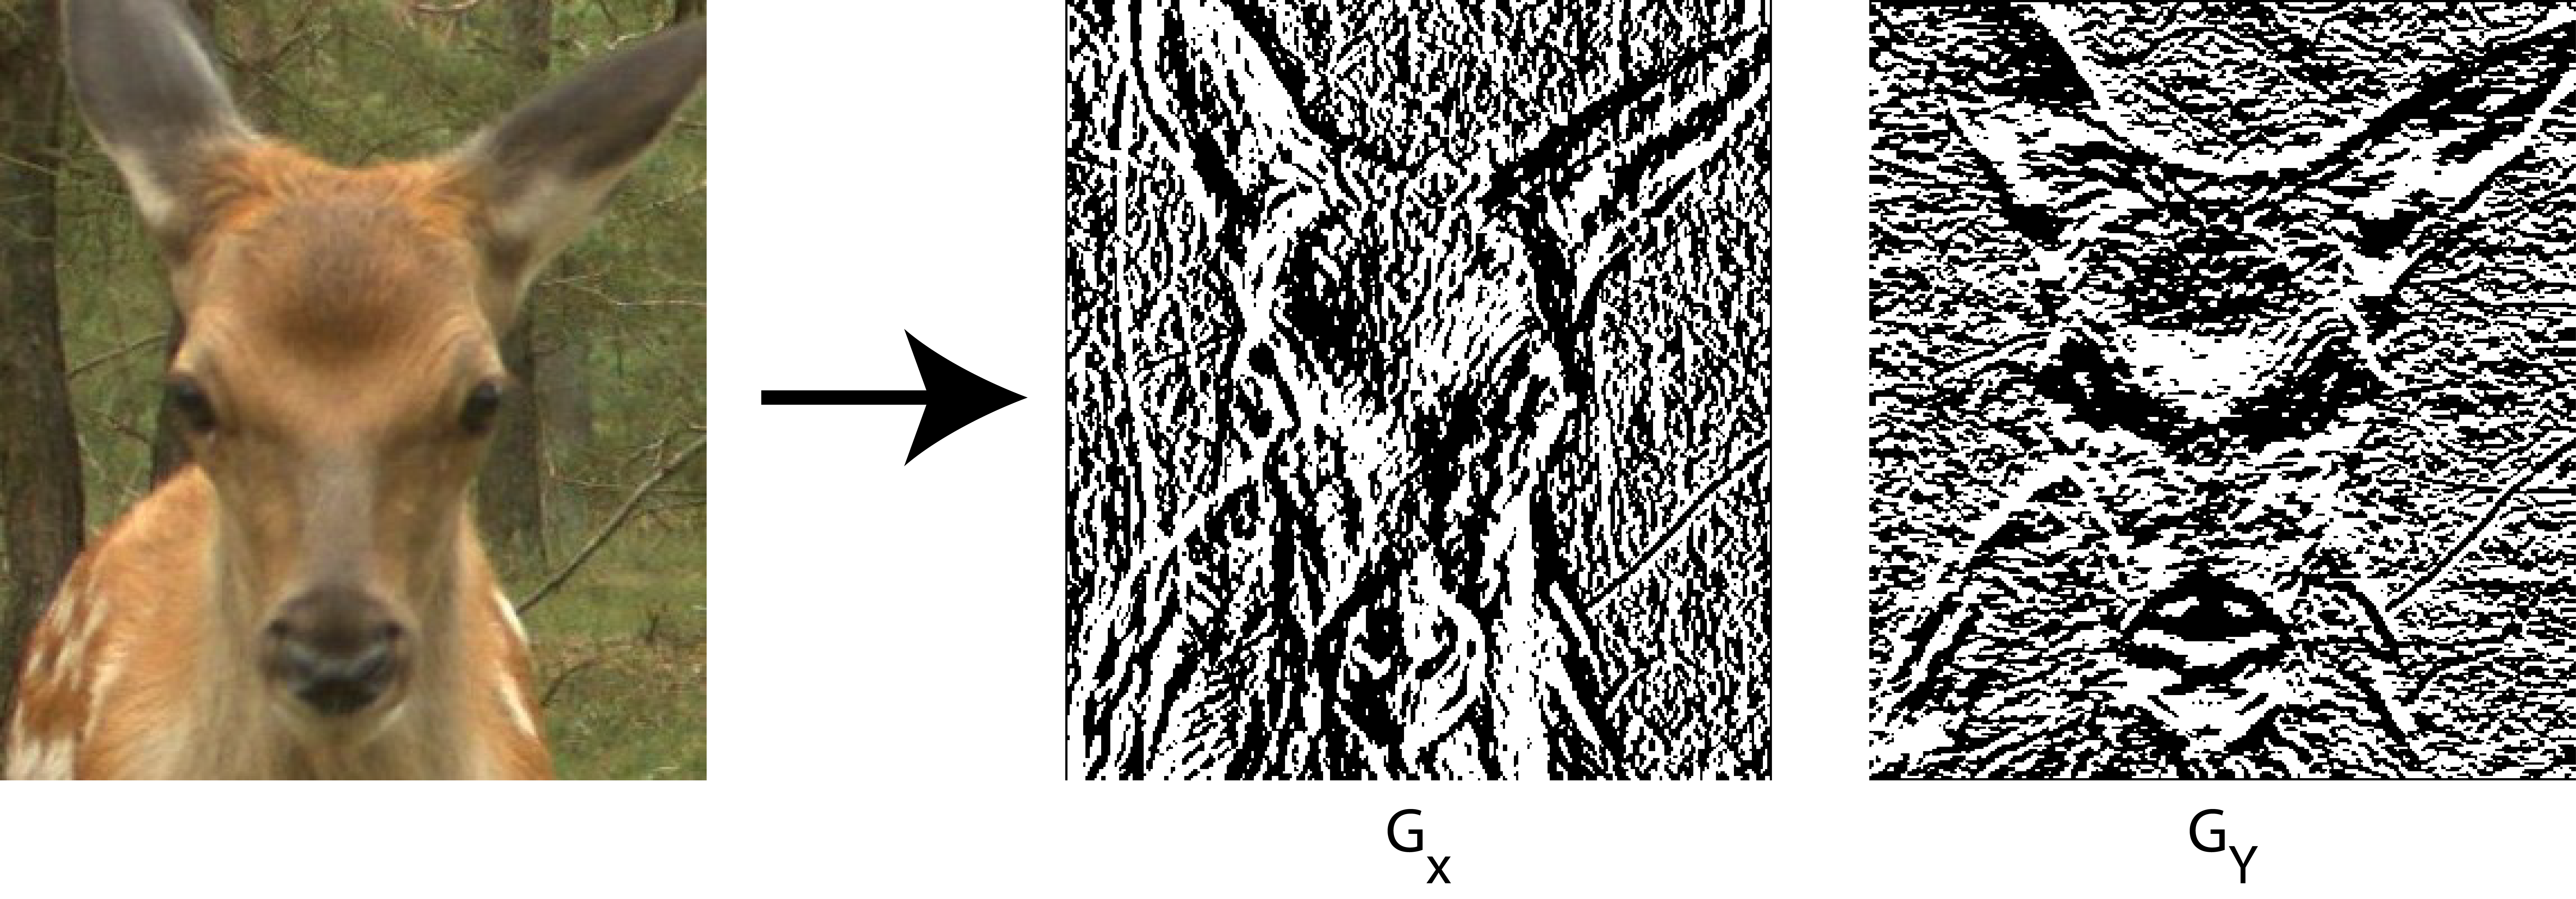
\includegraphics[trim={0 0cm 0cm 0cm},clip=true,width=13cm]{img/sobel.png}
\end{tabular}
\captionof{figure}{Exemplarische Ergebnisbilder des Sobel-Operators für die vertikale und horizontale Bild Achse. Die Grauwerte entsprechen der Magnitude des Gradienten.}
\label{fig:sobel}
\end{center}

Für jeden Pixel eines Bildes wird die Magnituden und Orientierung berechnet. Anschließend werden sie entsprechend ihrer Orientierung in gleich Gruppen sortiert. Häufig wird die Richtung der Orientierung ignoriert und 9 Gruppen verwendet. Durch das Ignorieren der Richtung wird also nur ein halber Kreis betrachtet (0 - 180°). Bei 9 Gruppen bedeutet dies, dass jede Gruppe 20° abdeckt. Der Wert dieser Gruppe ist dann die Summe aller Magnituden der Pixel die dieser Gruppe zugewiesen wurden. Es ist jedoch auch möglich andere Einteilungen zu verwenden. 
Formal ist ein solche Histogramm aus 9 Werten bereits ein HOG. Allerdings ist der Informationsgehalt dieser Repräsentation sehr gering. Um den Informationsgehalt zu erhöhen wird das Bild stattdessen systematisch in gleich große Bereiche unterteilt und für jeden Bereich ein Histogramm gebildet. Diese Histogramme werden abschließend konkateniert und als ein HOG-Deskriptor verwendet. Durch die Unterteilung werden Informationen der einzelnen Bildbereich bewahrt und somit kann ein Bild wesentlich besser beschrieben werden. Die systematische Unterteilung des Bildes wird wir folgt durchgeführt. Das Bild wird in gleich große Zellen unterteilt, so das jeder Pixel in genau einer Zelle enthalten ist (siehe Abbildung~\ref{fig:sobel2hog} rotes Raster). Anschließend werden jeweils vier dieser Zellen zu einem Block zusammengefasst (siehe Abbildung~\ref{fig:sobel2hog} grünes Rechteck) und für jeden dieser Blöcke wird nach dem \textit{Sliding Window} Prinzip eine Histogramm erstellt. Dies bedeutet das jeder Zelle (alle außer die Randzellen) vier mal in einem HOG repräsentiert werden. Diese wird daher gemacht, da es so möglich ist jedes Block HOG zu normalisieren, aber durch die Normalisierung nicht der Kontext zu den umgebenen Zellen verloren wird. 
Ein vollständiges HOG, bestehend aus den Konkatenation der Teil-Histogramm ist in Abbildung~\ref{fig:img2HOG} gezeigt. In der Gradienten Darstellung ist das gezeigte Reh noch leicht zu erkennen, da der Deskriptor deutlich die Kanten des Tieres hervorhebt. Diese veranschaulicht gut das die essentiellen Informationen erhalten bleiben obwohl die Datenmasse stark reduziert wurde. \cite{hog1}
\begin{center}
\begin{tabular}{c}
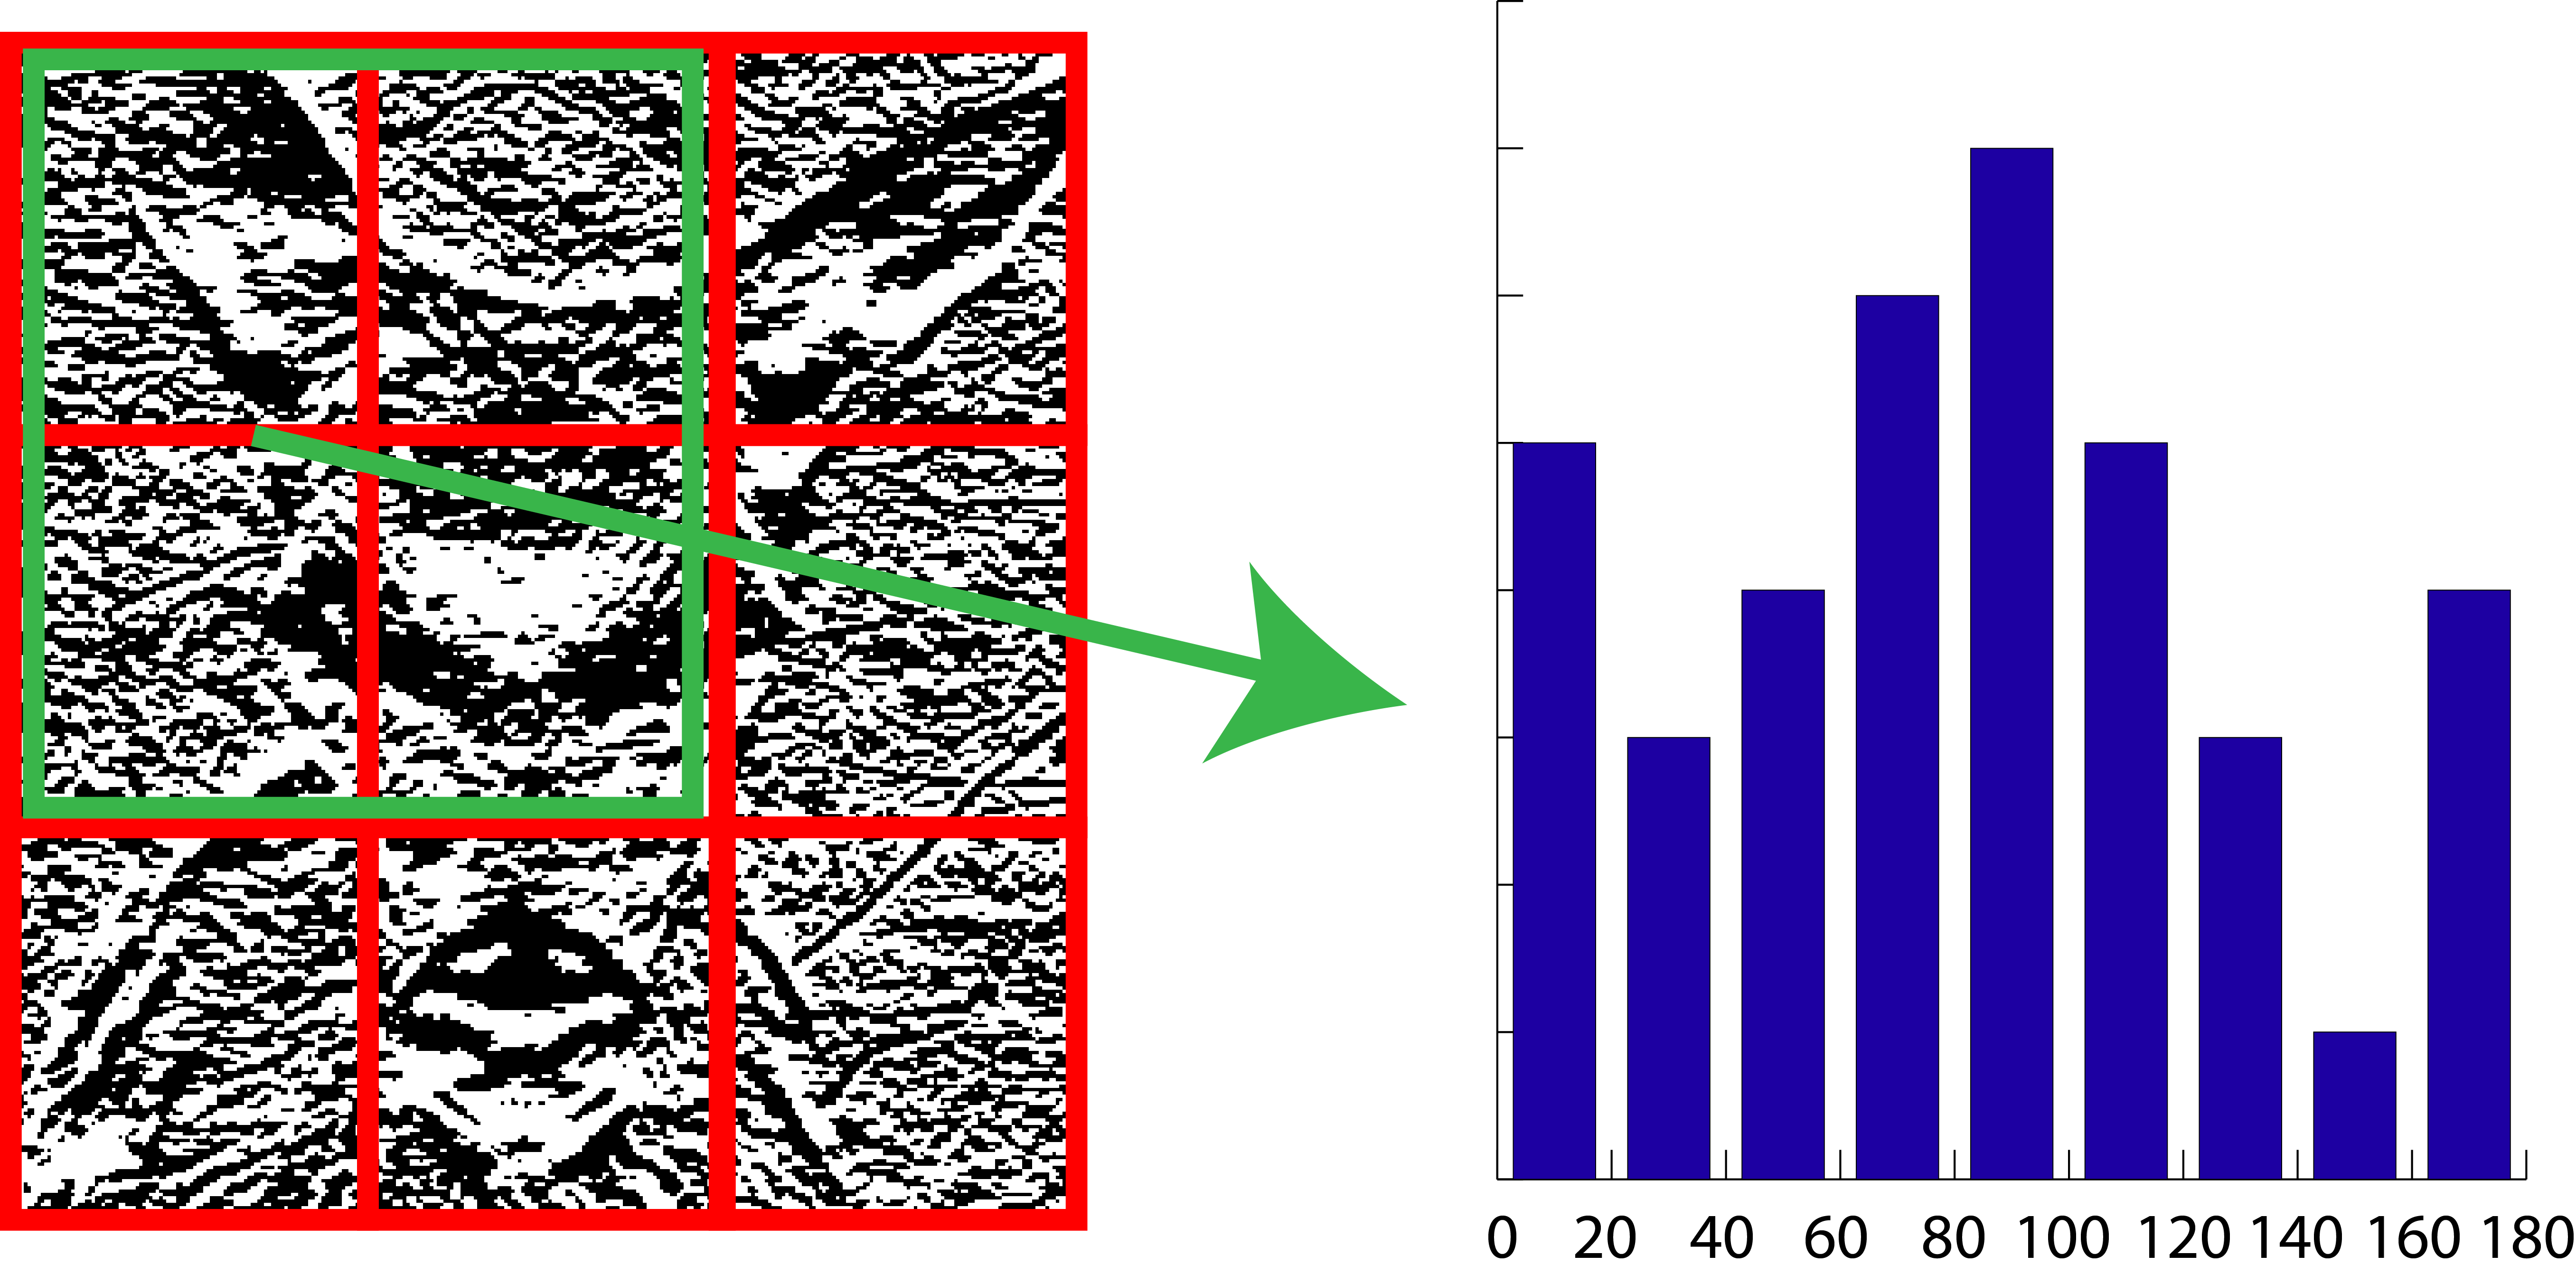
\includegraphics[trim={0 0cm 0cm 0cm},clip=true,width=13cm]{img/sobel2hog.png}
\end{tabular}
\captionof{figure}{Veranschaulichung der Erstellung eines HOG-Deskriptor. Das rote Raster visualisiert die Unterteilung in Zellen. Jeweils vier dieser Zellen werden zusammen als Block betrachtet. So das hier 4 Blöcke möglich wären. Für jeden Block kann dann ein normalisiertes Histogramm erstellt werden. Hier exemplarisch für den grünen Block gezeigt.}
\label{fig:sobel2hog}
\end{center}

\begin{center}
\begin{tabular}{c}
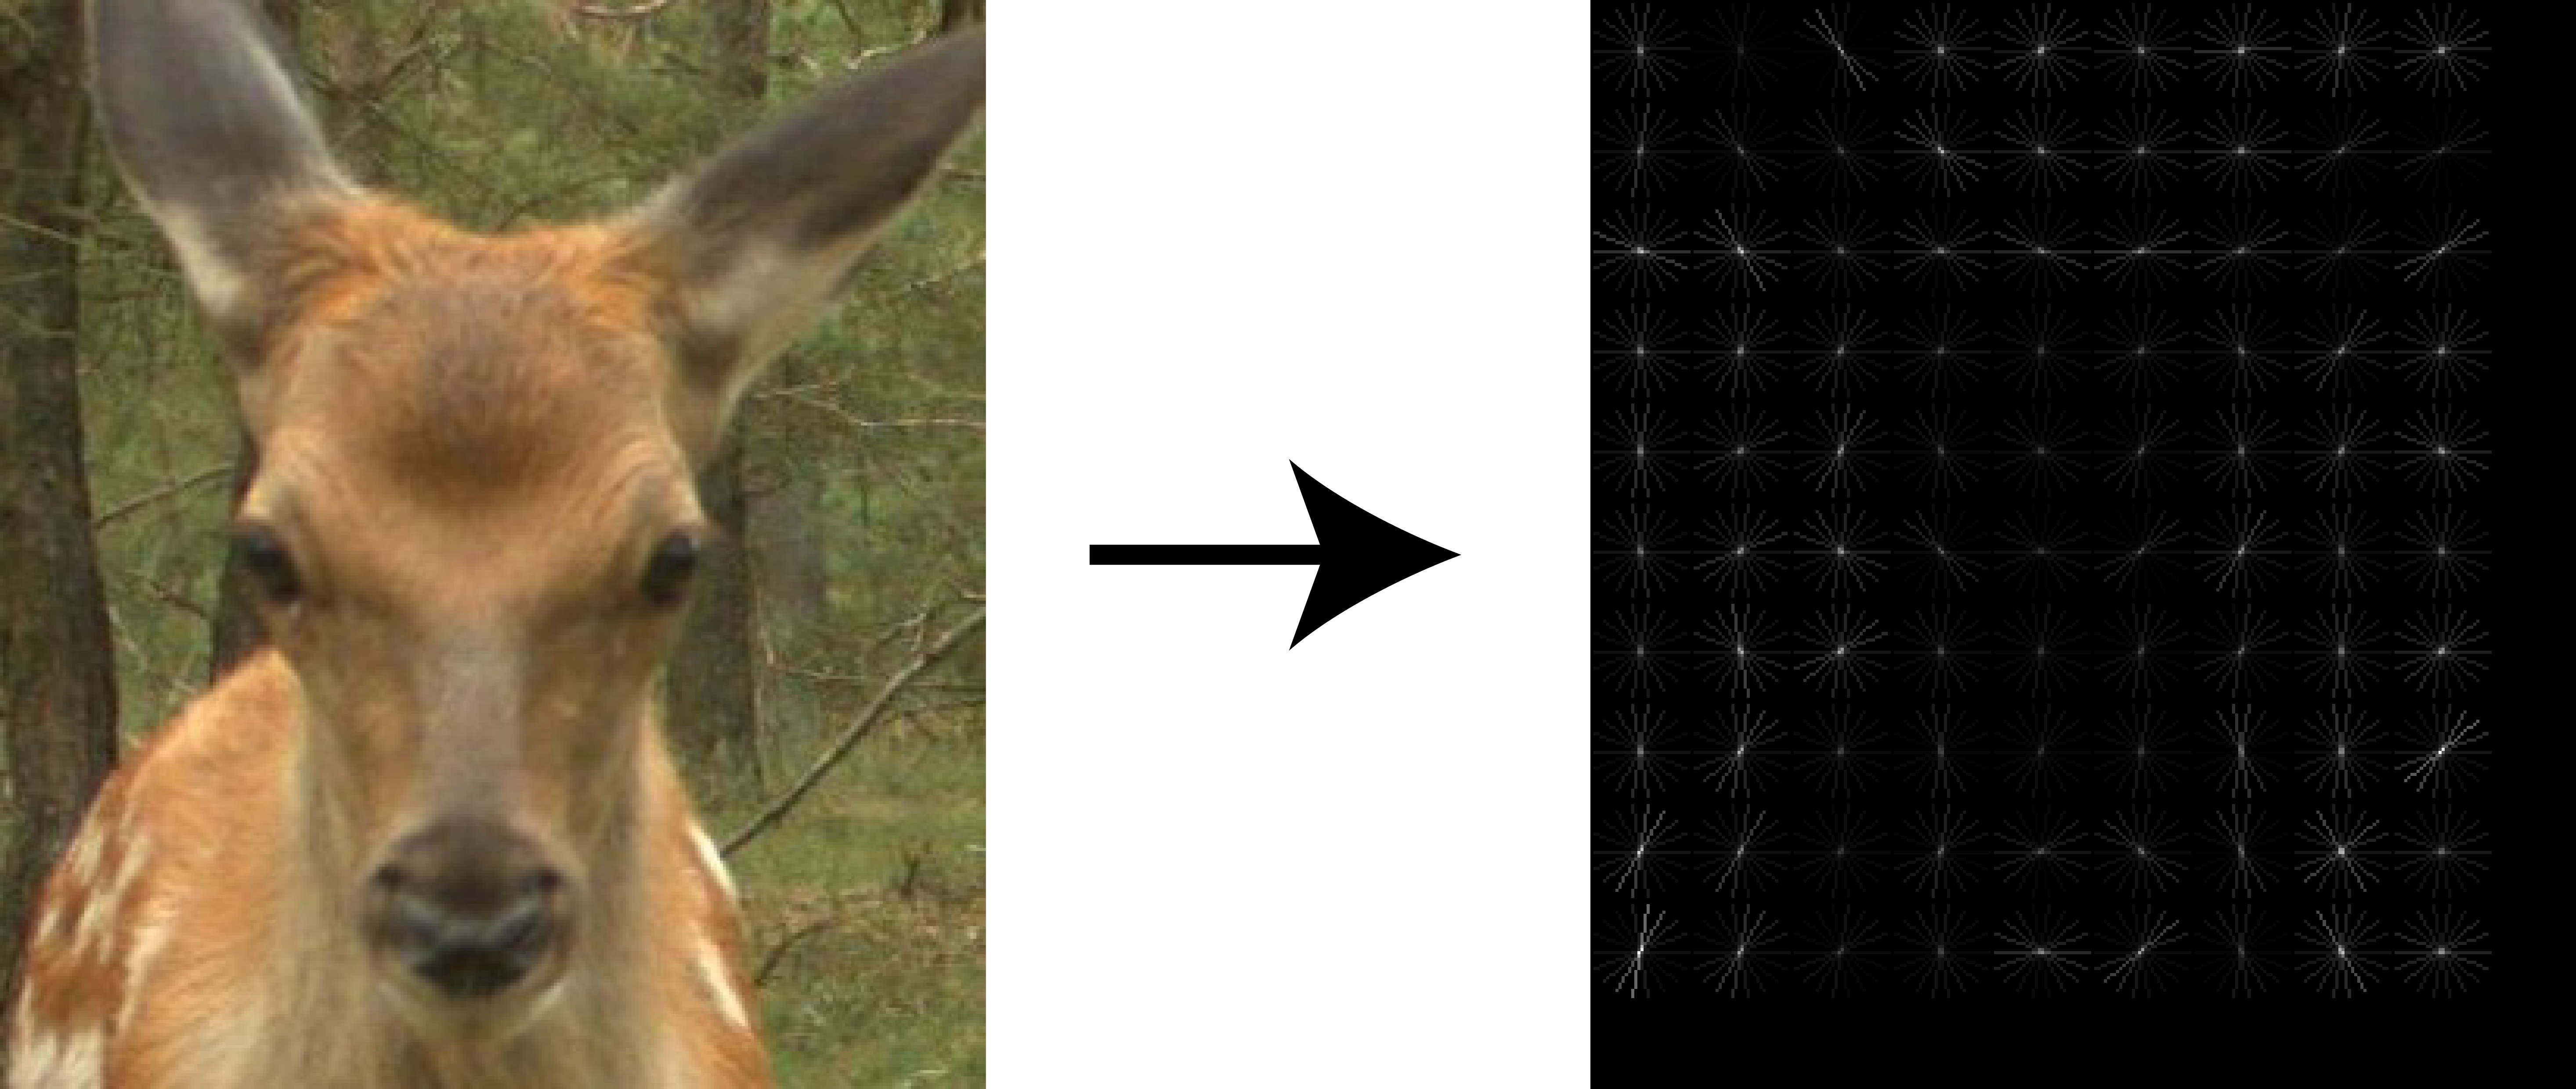
\includegraphics[trim={0 0cm 0cm 0cm},clip=true,width=13cm]{img/Img2HOG.png}
\end{tabular}
\captionof{figure}{Exemplarischer Bildausschnitt (links) und die visuell aufbereitet Repräsentation als HOG-Deskriptor (rechts). In der HOG Repräsentation ist es immer noch möglich das Reh zu erahnen.}
\label{fig:img2HOG}
\end{center}

\begin{center}
\begin{tabular}{c}
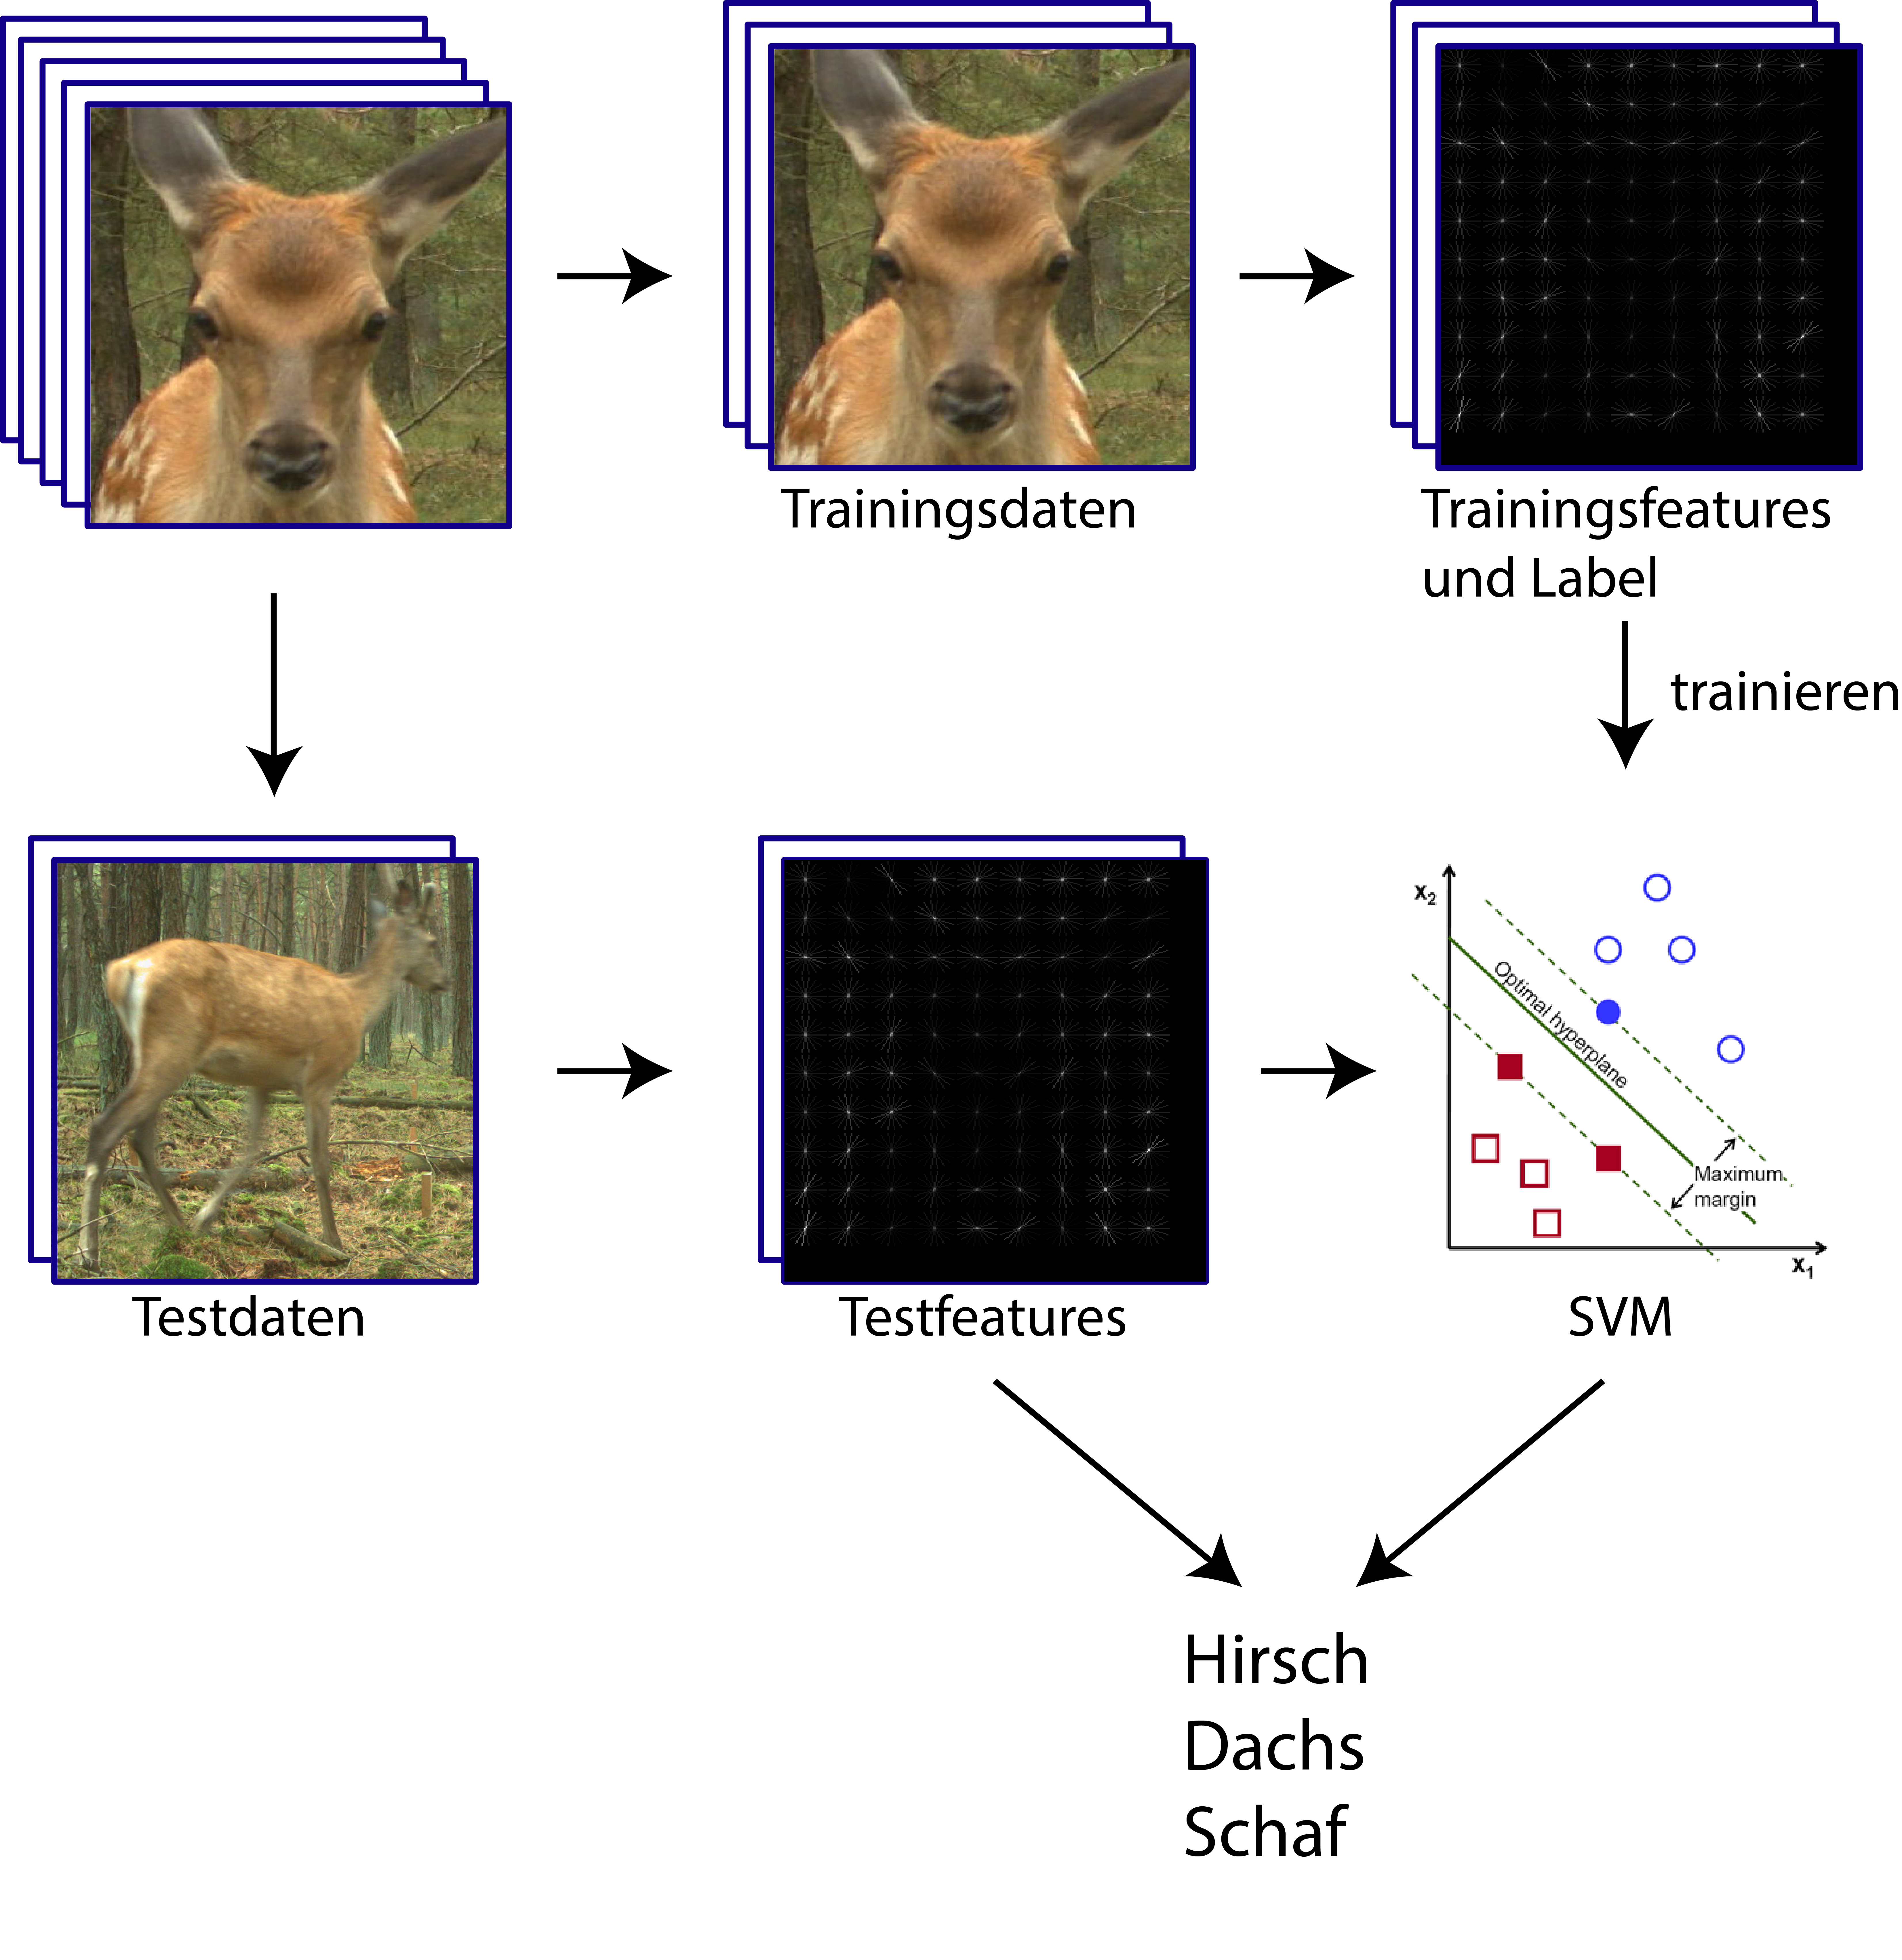
\includegraphics[trim={0 0cm 0cm 0cm},clip=true,width=13cm]{img/ClassificationOverview.png}
\end{tabular}
\captionof{figure}{Exemplarische Ergebnisbilder des Sobel Operators für die vertikale und horizontale Bild Achse. Die Grauwerte entsprechen der Magnitude des Gradienten.}
\label{fig:hog_classification_ov}
\end{center}

2) Wie wird es bestimmt?

3) Implementierung von OpenCV/Parameter Erklärung

\subsection{Implementierung}

\subsubsection{Optimierung und Auswertung}


